%%%%%%%%%%%%%%%%%%%%%%%%%%%%%%%%%%%%%%%%%%%%%%%%%%%%%%%%%%%%%%%%%%%%%%%%
%    INSTITUTE OF PHYSICS PUBLISHING                                   %
%                                                                      %
%   `Preparing an article for publication in an Institute of Physics   %
%    Publishing journal using LaTeX'                                   %
%                                                                      %
%    LaTeX source code `ioplau2e.tex' used to generate `author         %
%    guidelines', the documentation explaining and demonstrating use   %
%    of the Institute of Physics Publishing LaTeX preprint files       %
%    `iopart.cls, iopart12.clo and iopart10.clo'.                      %
%                                                                      %
%    `ioplau2e.tex' itself uses LaTeX with `iopart.cls'                %
%                                                                      %
%%%%%%%%%%%%%%%%%%%%%%%%%%%%%%%%%%
%
%
% First we have a character check
%
% ! exclamation mark    " double quote  
% # hash                ` opening quote (grave)
% & ampersand           ' closing quote (acute) 
% $ dollar              % percent       
% ( open parenthesis    ) close paren.  
% - hyphen              = equals sign
% | vertical bar        ~ tilde         
% @ at sign             _ underscore
% { open curly brace    } close curly   
% [ open square         ] close square bracket
% + plus sign           ; semi-colon    
% * asterisk            : colon
% < open angle bracket  > close angle   
% , comma               . full stop
% ? question mark       / forward slash 
% \ backslash           ^ circumflex
%
% ABCDEFGHIJKLMNOPQRSTUVWXYZ 
% abcdefghijklmnopqrstuvwxyz 
% 1234567890
%
%%%%%%%%%%%%%%%%%%%%%%%%%%%%%%%%%%%%%%%%%%%%%%%%%%%%%%%%%%%%%%%%%%%
%

\documentclass[12pt]{iopart}
%\documentclass[12pt]{article}
%\usepackage{amsmath}
%\usepackage{cite}
\usepackage{amssymb,amsfonts}
%\usepackage{algorithmic}
\usepackage{graphicx}
%\usepackage{textcomp}
\usepackage{xcolor}
%\usepackage{graphicx}
%Uncomment next line if AMS fonts required
%\usepackage{iopams}  
\begin{document}

\def\brian[#1]{{\color{red} #1 }}

\title[Heterogeneous Control of Cell Differentiation Dynamics]{Exploiting Intrinsic Noise to Achieve Heterogeneous Control of Cell Differentiation Dynamics in the Presence of Time Delays, Model Uncertainties, and Extrinsic Variability}
\maketitle

\author{M P May$^1$, B Munsky$^{1,2}$}

\address{$^1$ School of Bioengineering, Colorado State University, Fort Collins, CO, USA}
\address{$^2$ Department of Chemical and Biological Engineering, Colorado State University, Fort Collins, CO, USA}

\begin{abstract}
Previous research has focused on robust control performance in the presence of noise, but understanding controllers that exploit noise remains incomplete. 
Motivated by Maxwells-Demon, we previously proposed a difficult control problem which requires the exploitation of noise in a stochastic system to break symmetry between two signals. We found multiple such controllers which could exploit noise to break symmetry between two cells under a variety of system information.
This work extends that analysis to include stochastic systems that trace a moving target, are affected by time delay, intrinsic noise, or measurement uncertainty.
 We find that noise-exploiting controllers can remain highly effective despite coarse approximations to the model's scale or incorrect estimations of key model parameters, and these controllers can even retain performance for significant time delays.  Together, these findings suggest that noise-exploiting control should be possible where models are always approximate, where parameters are always uncertain, and where observations are corrupted by errors.


\end{abstract}
Keywords: Stochastic Control, Gene Regulation, Optogenetics

%
% Uncomment for keywords
%\vspace{2pc}
%\noindent{\it Keywords}: Stochastic control, optogenetic, synthetic biology
%
% Uncomment for Submitted to journal title message
%\submitto{\JPA}
%
% Uncomment if a separate title page is required
\maketitle
% 
% For two-column output uncomment the next line and choose [10pt] rather than [12pt] in the \documentclass declaration
%\ioptwocol

\section{Introduction}
\begin{figure}
\begin{center}
\includegraphics[width=\columnwidth]{Cartoons.pdf}
\caption{{\bf Optogenetic control of multiple cells using a single light input.}
({\bf A}) Schematic of the light activated genetic system with autoregulation.
({\bf B}) Diagram of the stochastic SIMO control problem using two optogenetic cells sharing an input.
({\bf C}) Adapted from (PAPER). Noise exploiting controllers were optimized to a fully aware control input (I), and partially aware control input(III). Marginal distributions are solved using the finite state projection and show a break in symmetry using both controllers (II and IV) }
\label{cartoons}
\end{center}
\vspace{-0.3in}
\end{figure}
% XXX - Please modify figure as follows: (1) switch panels A and B to match caption. (2) Change title of panel B (previously panel A) to "External Observer, controller and actuator".  (3) Change title of panel A (previously panel B) to "Internal gene regulation pathway". (4) Change title of panel C to "Feedback control law and resulting performance"
% MMM - Made the edit

Uncertain fluctuations, or `noise,' is a common theme throughout many fields of engineering, and is a frequent concern when attempting to control any human-made system such as vehicles\cite{XXX}, production machinery\cite{XXX}, or chemical processes\cite{XXX}.
Noise arrises from many sources, occasionally from quantum events and thermally-induced fluctuations but more commonly from unknown or uncharacterized physical processes, and as such, these fluctuations usually cannot be efficiently reproduced or predicted using purely physical or mechanistic models.
Rather, statistical models are usually employed where key mechanisms or dynamics are subject to stochastic variations or inputs that act as a proxy for random or un-modeled fluctuations elsewhere in the system.
In this context, much effort has been placed on enhancing the robustness of controlled processes, where uncertain or unpredictable variations in internal or external parameters are modeled as intrinsic or extrinsic noise \cite{XXX}.
For many macroscopic, human-engineered systems, the resulting system dynamics can be modeled effectively simply by combining a deterministic (i.e., noise-free) model with additive noise (usually assumed to be Gaussian under arguments based on the central limit theorem)\ref{XXX}, and most current approaches seek to control the system to minimize variations that result from the noisy inputs. 

Analyses of noise and control theory are equally relevant to understand the basic biological processes of gene transcription regulation\cite{XXX} or mRNA translation regulation \cite{XXX} or to modify these processes for practical use\cite{XXX}.
However, at this mesoscopic scale of cellular biology, where transcription factors compete to activate or deactivate individual genes or where mRNA or protein molecules are present at just a few copies (or none at all) per cell, additive noise model is far less realistic.
In this case, Brownian motion, discrete stochastic gene regulation, and noisy mRNA dynamics collectively generate a fundamentally stocastic environment that cells must effectively manage. 
At this scale, the order or timing of a single reaction event (e.g., the binding of a transcription factor to a promoter) can have dramatic consequences that could last for several cellular generations (e.g., the activation or repression of a gene that promotes unfettered cell growth and differentiation). 
The cell's drive towards homeostasis requires dealing with the inherently chaotic and noisy processes that reside within it, and despite these challenges, cells generally demonstrate strong capability to survive these noisy processes. 
When seeking to understand how such systems evolve or react, the central limit theorem and the Gaussian noise may not apply, and a more detailed statistical analysis of probabilistic behavior is needed uncover hidden properties of cellular control mechanisms.

One emerging field that is particularly dependent on the integration of control and noise is synthetic biology, which aims to develop modular\cite{Ng2019} and orthogonal \cite{Liu2018} components to sense and manipulate \cite{Sheets2020} complex logical systems, enabling them to exhibit a wide range of advanced biological behaviors\cite{Shin2020}. 
Advances in optogenetics have enhanced the ability to reliably actuate embedded systems within cells, offering the potential to exert precise temporal and spatial control on cellular components\cite{Sheets2020,Baumschlager2017,Chen2020,Lillacci2018}.
These developments have facilitated computer-programmable regulation of cellular protein production through external optogenetic inputs and smart microscope techniques\cite{Fox2021,Baumschlager2021,Lugagne2017}. 
These digital-synthetic actuators enable fine-tuned, computer-modulated control of cellular systems, previously unattainable, with faster response times compared to chemical diffusion\cite{Rullan2018, Baumschlager2017} . 
Classical and modern control methods like PID control and model predictive control have been implemented in such systems\cite{} to control synthetic systems to different stable points. 
% XXX Missing Citation above.

While most previous control efforts focussed on deterministic ordinary differential equation (ODE) formulations of the control problem, a few pioneering theoretical works have extended these analysis to include noise and have used stochastic simulations to show how systems can be guided towards unstable points by oscillating around those points \cite{Guarino2020}. 
It has recently been shown that new control techniques that leverage the complete probability distribution information of the system could actually harness the noise of single-cell gene regulation to achieve more complicated control objectives. 
For example, inspired by the genetic toggle switch from Kobayashi et al.\cite{Kobayashi:2004}, Szymanska et al.~\cite{Szymanska2015} showed that noise could be exploited to achieve independent control of multiple cells using a single input, even despite uncertain parameters or time delays due to maturation of fluorescent proteins or limited observation of the regulatory proteins. 
In May et al.~\cite{May2021}, we identified a simplified stochastic model to reproduce data measured in Baumschlager, et al.\cite{XXX} for the expression from the XXX promoter under the optogenetic control of a UV-activated T7 polymerase (see model in Figure\ \ref{cartoons}A, top promoter).
We then proposed the addition of a positive auto-regulation (Figure\ \ref{cartoons}A, bottom promoter) to help maintain an elevated expression phenotype in the presence of UV excitation, and we demonstrated how a Single-Input-Multiple-Output (SIMO) multicellular controller could control multiple cells to arbitrary phenotypes using only a single input. 

%The solutions of the controllers was carried out by solving the chemical master equation (i.e., the forward Komogorov equation) to estimate the probability of possible cellular states. For a two cell, single-input-single output (SIMO) control problem, the FAC performed the best (figure\ \ref{cartoons}C(top)), and the PAC (figure\ \ref{cartoons}C(bottom)) 2nd, and pMPC controllers 3rd. In all cases, the controller's knowledge and explicit treatment of intrinsic noise was critical to improve the control performance, break symmetry, and enable the SIMO control of all cells.

This paper extends the analysis of the SIMO multicellular control problem by examining the impact of model uncertainties and fluctuating control objectives on the control performance. 
These uncertainties include coarse-grained approximations of the system dynamics, errors or extrinsic variations in the system parameter, and time delays between the observation of the cellular dynamics and actuation of the control process. 
In the following `Methods' we introduce our formulation of the chemical master equation to analyze the discrete stochastic distribution of cellular responses; we define multiple controllers and demonstrate the computation of their effects on cell dynamics; and we show how the control law can be optimized to improve performance.
In the `Results' section, we explore the how model approximations, parameter inaccuracies, and time delays affect control performance, and we demonstrate a simple scheme for controlling cells to track a dynamically changing reference signal. 
Using discrete stochastic models based on the chemical master equation, we demonstrate that combining biochemical noise, nonlinear auto-regulation, and a single optogenetic feedback could control two genetically identical cells with different initial conditions to follow different desired trajectories at different frequencies and phases. 

%Figure\ \ref{cartoons}C(left) presents heat maps for two control laws, which a single external UV excitation signal based on observed cellular state.  Figure\ \ref{cartoons}C(right) shows the corresponding achievable marginal stationary distributions. Effective control was possible with both Fully Aware Feedback Controllers (FAC, Figure\ \ref{cartoons}C(top)) and Partially Aware Feedback Controllers (PAC, Figure\ \ref{cartoons}C(bottom)), even when the control model was an approximate simplification of the actual process dynamics.

\section{Methods}
In May et al. \cite{May2021}, we developed two models for the description of an optogenetically controlled gene expression system.
These first model consisted of six species to describe the light-activated association of two T7 split domains (species 1 and 2) which combine to form an active T7 polymerase (species 3) under optogenetic excitation. 
The active polymerase could then associate with inactive T7 promoters (species 4), resulting in the formation of an active allele (species 5) that could then transcribe and translated to produce the desired protein product (species 6). 
The second, much simpler, single-species model was developed by assuming quasi-steady equilibrium for the first five species. 
Both models were independently parameterized using the same experimental data from Baumschlager et al. \cite{XXX}. 
Furthermore, an extension was made to each model to incorporate a secondary self-activated promoter-gene construct, where the expression rate was determined by a Hill function \ref{prodRate}.
Through simulations, we showed that a feedback control law could be designed to force multiple cells to different and individually chosen equilibrium states using a single optogenetic control signal. 
We also showed that when this control law was parametrized using the simple model, it could be used effectively to control the behavior of the more complicated system, thus demonstrating that control performance could remain high despite inaccuracies in the model.
In the current work, we adopt the simpler of the two models and extend our analyses to consider the effects of additional model inaccuracies, including coarse-grained model approximations, parameter errors, and time delays, and we also explore the possibility that a single optogenetic control signal could drive the system to track temporally-changing reference signals.
Section \ref{sec:Model} introduces the model; Section \ref{sec:Stochastic} develops a Master Equation description of the models probabilistic dynamics; Section \ref{sec:Quantification} defines a control objective and optimizes that metric to obtain a baseline control law; and finally Sections \ref{sec:Scaling} and \ref{sec:Delay} introduces uncertainties into the model related t the granularity of the model approximation or the introduction of time delays, respectively. 

\subsection{Model}\label{sec:Model}
To assess the impact of model approximations on the implementation of noise-enhanced control strategies, we begin with the one-species model proposed by May et al. \cite{May2021} (Fig. \ref{cartoons}A). 
This model comprises two reactions for production and degradation of the key protein. 
The nonlinear, UV-dependent production is defined by the following equation:
\begin{equation}
\nu_1(x,t)= \kappa\frac{x^\eta}{x^\eta+\beta^\eta}+ k_0 + u(UV(t)),
\label{prodRate}
\end{equation}
%
%These model dynamics were then simplified to a single ODE with auto-regulation describing the protein accumulation as: 
%\begin{equation}
%\frac{dp}{dt}=u(x_1,x_2)  + \kappa\frac{p^\eta}{p^\eta+\beta^\eta}+ k_0 -\gamma p,
%\label{rateeq}
%\end{equation}
%
where $x$ is the instantaneous protein level; $\kappa$ is the maximum strength of the auto-regulation promoter; $\beta$ is the concentration at which auto-regulation promoter reaches its half maximal strength; $\eta$ is the cooperativity in the auto-regulation promoter; $k_0$ is the leakage rate from both promoters; and $u(UV(t))$ is the UV-dependent strength of the T7 promoter. 
Feedback enables the external modulation of the light input using the state of the system, thereby controlling the T7 promoter strength as a function of state rather than time and eliminating the explicit time dependance in $u(UV(t))$.
Protein degradation is assumed to be a first order process with rate $\gamma$:
\begin{equation}
\nu_2(x) = \gamma x.
\end{equation}
All baseline parameters describing the auto-regulation promoter, $\kappa$, $\eta$, $\beta$, and $k_0$, and the degradation rate $\gamma$ are presented in Table 1~\cite{May2021} and are fixed throughout the current study.

\begin{table}[]
\caption{Baseline Model Parameters}
\begin{center}
\begin{tabular}{|c|c|c|}
\hline
Parameter & Value   & units                     \\ \hline \hline
$\kappa$         & 0.406   & 1/min \\ \hline
$\beta$          & 20.0    & Molecules            \\  \hline
$\eta $           & 8.00    & unitless          \\  \hline
$k_0$           & 0.0001  & 1/min \\  \hline
$\gamma$         & 0.0203  & 1/min         \\  \hline
$u$              & dynamic & 1/min \\ \hline
\end{tabular}
\label{table}
\end{center}
\vspace{-0.2in}
\end{table}

\subsection{Stochastic analyses of the model}\label{sec:Stochastic}
To describe the discrete stochastic behavior of the above model for a population system with $N_{\rm c}$ cells, we define the current state of the system as the tuple of the non-negative numbers of proteins in each cell: $\mathbf{X}_i = [x_{1},x_{2},\ldots,x_{N_c}]_i\in \mathbb{Z}_{\ge 0}$, where the index $i$ denotes the enumeration of the state within the countably infinite set of all possible states, $\mathbf{X}_i\in\mathcal{X}=\{\mathbf{X}_1,\mathbf{X}_2,\ldots\}$.
The stoichiometry vector, $\mathbf{s}_{\mu}$, for reaction number $\mu$ is then defined as the change in state following that reaction event (e.g., $\mathbf{X}_i \rightarrow \mathbf{X}_i + \mathbf{s}_\mu$). Specifically, the $2N_c$ possible reactions are defined in pairs corresponding to production ($\mu\in\{1,3,5,\ldots\}$) and degradation ($\mu\in\{2,4,6,\ldots\}$) as:
\begin{eqnarray}
\mathbf{s}_1 &= \mathbf{e}_1,\ \mathbf{s}_2 = -\mathbf{e}_1,\nonumber\\ 
\mathbf{s}_3 &= \mathbf{e}_2,\ \mathbf{s}_4 = -\mathbf{e}_2,\nonumber\\
&\vdots \nonumber\\ 
\mathbf{s}_{\rm 2N_c-1} &= \mathbf{e}_{\rm N_c},\ \mathbf{s}_{\rm 2N_c} = -\mathbf{e}_{\rm N_c}, \label{Stochs}
 \end{eqnarray}
where each $\mathbf{e}_{i}\in\mathbb{Z}^{{\rm N_ c}}$ is is a Euclidean vector (i.e., unity for the $i^{\rm th}$ entry and otherwise zero). The corresponding propensity functions are:
\begin{eqnarray}
w_1(\mathbf{X}) &= u(\mathbf{X},t)  + \kappa \frac{x_1^\eta}{x_1^{\eta}+\beta^{\eta}} + k_0,\ w_2(\mathbf{X}) = \gamma x_1,\nonumber\\
w_3(\mathbf{X}) &= u(\mathbf{X},t)  + \kappa \frac{x_2^\eta}{x_2^{\eta}+\beta^{\eta}} + k_0,\ w_4(\mathbf{X}) = \gamma x_2,\nonumber\\
&\vdots \nonumber\\
w_{\rm 2N_c-1}(\mathbf{X}) &= u(\mathbf{X},t)  + \kappa \frac{x_N^\eta}{x_N^{\eta}+\beta^{\eta}} + k_0,\ w_{\rm 2N_c}(\mathbf{X}) = \gamma x_N.\label{Props}
 \end{eqnarray}

These definitions of the stoichiometry and propensity functions allow us to implement the Gillespie stochastic simulation algorithm (SSA) \cite{Gillespie1992, Gillespie1977} to generate representative trajectories of the stochastic process. At each step two random numbers are generated to determine the time and the type of the next reaction. Given the current state $\mathbf{X}$, the time until the next reaction is distributed according to an exponential random with rate parameter equal to the inverse of the sum of the propensity functions:
\begin{equation}
Pr(\delta t = \tau) = \sum w_i(\mathbf{X}) \exp\left(- \sum{\mu=1}^{2N_c-1} w_\mu(\mathbf{X})\tau\right),
\end{equation}
and an instance of this random variable, $\delta t$,  can be sampled from this distribution using the expression:
\begin{equation}
\delta t = -\log\left(r_1 \sum_{\mu=1}^{2N_c-1}  w_\mu(\mathbf{X})\right),
\end{equation}
where $r_1$ is a uniform random variable between zero and one.
The probability of for the specific individual reaction $R_k$ to fire from all possible reactions is given by:
\begin{equation}
Pr(R_k)=\frac{w_k}{\sum w_{\mu=1}^{2N_c-1} (\mathbf{X})},
\end{equation}
and thus the reaction that fires at time $t+\tau$ is a categorical random variable pulled from $Pr(R_k)$.  The SSA is then simulated by stepping through time one reaction at a time and updating the state of the system by adding the stoichiometry of the reaction to the state of the system.

However, a more direct analysis of the chemical master equation (CME) is necessary for performance quantification and optimal controller design. The high dimensional CME is a linear ODE that describes the time-dependent changes in probability mass of all possible states. Using the specified reaction propensities and stoichiometries, the CME can be expressed as:
\begin{equation}
\frac{d}{dt}P(\mathbf{X}_i)=\sum_{\mu=1}^{2{\rm N_c}}
\left(
-w_{\mu}(\mathbf{X}_i)P(\mathbf{X}_i)
+w_{\mu}(\mathbf{X}_i-\mathbf{s}_{\mu})P(\mathbf{X}_i-\mathbf{s}_{\mu})
\right).\label{CMEindex}
\end{equation}
For convenience, the CME can also be formulated more compactly in matrix-vector form as:
\begin{equation}
\frac{d}{dt}\mathbf{P}=(\mathbf{A}_0+\textbf{Bu}^{\mathcal{C}})\mathbf{P},\label{CME}
\end{equation}
where $\mathbf{P} = [P(\mathbf{X}_1), P(\mathbf{X}_2), \ldots ]^T$ is the enumerated probability mass vector for all possible states of the system; $\mathbf{A}_0$ is the infinitesimal generator of the stochastic process due to the autoregulation promoter and degradation events;  $\textbf{u}^{\mathcal{C}} =[u^{\mathcal{C}}(\mathbf{X}_1), u^{\mathcal{C}}(\mathbf{X}_2), \ldots ]^T$ is the collection of control inputs associated with each state; and $\textbf{Bu}^{\mathcal{C}}$ is the contribution that these control inputs make to the infinitesimal generator when included into the feedback process. 
 
More specifically, the zero-control infinitesimal generator, $\mathbf{A}_0$, is constructed according to:
\begin{equation}
[\mathbf{A}_0]_{ij} = \left\{
\begin{array}{rl}
-\sum_{\mu =1}^{2N_{\rm c}} w_{\mu}(\mathbf{X}_j), &\textrm{for }i=j,\\
w_{\mu}(\mathbf{X}_j), &\textrm{for }\mathbf{X}_i = \mathbf{X}_j+\mathbf{s}_\mu\\
0, & \textrm{otherwise,}
\end{array}\right. 
\label{InfA}
\end{equation}
and the feedback infinitesimal generator, $\mathbf{Bu}^{\mathcal{C}}$, of the controller is constructed according to
\begin{equation}
[\mathbf{Bu^{\mathcal{C}}]}_{ij} = \left\{
\begin{array}{rl}
- N_{\rm c}{u}^{\mathcal{C}}(\mathbf{X}_j), &\textrm{for }i=j\\
{u}^{\mathcal{C}}(\mathbf{X}_j), &\textrm{for }\begin{array}{ll}\mathbf{X}_i =\mathbf{X}_j + \mathbf{e}_{i_{\rm c}}, \\ \textrm{and } i_{\rm c} = 1,\ldots,N_{\rm c}\end{array},\\
0, & \textrm{otherwise,}
\end{array}\right.
\label{InfB}x
\end{equation}
where ${u}^{\mathcal{C}}(\mathbf{X}_j)$ is the specification of the controller, $\mathcal{C}$, in terms of the current instantaneous state, or its partial observations.

For a given controller, the equilibrium distribution of the system ($\mathbf{P}^*$) can be found by solving Eq.\ \ref{CME} and is given by:
\begin{equation}
\mathbf{P}^*={\rm null}(\mathbf{A}+\textbf{Bu}^{\mathcal{C}}).\label{SSDist}
\end{equation}


In principle, the master equation in Eq.\ \ref{CME} could contain an uncountably infinite number of states, and therefore the exact solution as well as the null vector in Eq.\ \ref{SSDist} may not be computable exactly.  To address this issue, we first truncate the system at a finite number for each species and then apply a reflecting boundary condition, resulting in a finite dimensional master equation. To assess the time interval over which this truncation is valid, we also solve the Finite State Projection\cite{Munsky:2006} for the same truncation, which allows us to compute an upper bound on the truncation error as a function of time. 

\brian[We should use the FSP to compute the error of the truncation for a couple cases.  We can talk about how to do this when we meet.]

%Finite state projections are a powerful way to simulate master equation analysis which enables the assessment of simulation accuracy, but these simulations have challenges measuring the steady state of the system since all probability will always enter error at long enough time scales. To enable control of steady state systems, a truncated FSP which reflects probability back into the system enables this calculation.

\subsection{Quantification and optimization of control performance}\label{sec:Quantification}
In the SIMO control of stochastic processes, a single input is applied simultaneously to all systems at once and a control signal that acts beneficially on one system destabilizes other systems. Stochastic SIMO control inputs which seek to control cells one-cell-at-a-time create increased instability and response variability in the other signals not being controlled.
Thus, even in systems which do a good job at controlling a system cannot independently control individual cells to a desired target point without impacting the variance of others, so an effective controller must strike a balance among the desired behaviors of all cells in the system. 

To quantify performance success, we define the {\em steady state performance error}, $J$, as the expected steady state Euclidean distance of the process from the specified target state, $\mathbf{T}$:
 \begin{equation}
 J = \mathbb{E}\{|\mathbf{X}-\mathbf{T}|_2\}.
 \end{equation}
The squared score is easily calculated by applying a linear operator on steady state probability distribution $\mathbf{P}^*$ (Eq.\ \ref{SSDist}) as follows:
\begin{eqnarray}
J^2&= \lim_{t\rightarrow \infty}\mathbb{E}\{|\mathbf{X}(t)-\mathbf{T}|_2^2\}, \nonumber \\ 
&=\sum_{i_1,i_2,\ldots} P^*(x_1=i_1,x_2=i_2,\ldots) \left[(i- T_1)^2 + (j- T_2)^2 +\ldots\right],\nonumber  \\
&=\mathbf{C}\mathbf{P}^*,
\label{Euclid}
\end{eqnarray}
where $\mathbf{C}$ is simply a vector that contains the squared Euclidian distance of each state from the specified target T, i.e., $C_i = |\mathbf{X}_i-\mathbf{T}|_2^2$. 
As a result of this calculation, $J$ is a non-negative scalar that is zero if any only if $\mathbf{P}^*$ is a delta distribution located exactly at the target vector $\mathbf{T}$.

We consider two controller designs: the fully aware controller ($\mathbf{u}^{FAC}$) that bases its control signal on simultaneous protein count observations from both cells, and the partially aware controller ($\mathbf{u}^{PAC}$) that relies only on observations from a single cell:
\begin{equation}
\mathbf{u}^{FAC}=u(x_1,x_2),
\end{equation}
\begin{equation}
\mathbf{u}^{PAC}=u(x_2),
\end{equation}
where $x_1$ and $x_2$ are discrete integers greater than or equal to zero that represent the number of proteins in cell one and cell two. Despite their differences in their observation data, both the FAC and the simpler PAC are optimized to achieve the same goal, namely to drive both cells to their respective set points.

Optimization of $\mathbf{u}^{FAC}$ was performed using a gradient descent method to minimize $J$. Since the square root is a monotonically increasing function, minimizing $J^2$ results in the same control as would minimizing $J$ directly. Therefore, we calculate the negative gradient $-\frac{d(J^2)}{d\mathbf{u}^{FAC}}$ and walking in a small step $du$ in that direction. The calculation of the gradient is given by
\begin{equation}
\frac{d(J^2)}{d\mathbf{u}^{FAC}}=C \frac{dP}{d\mathbf{u}^{FAC}}
\end{equation}
Where $\frac{dP}{d\mathbf{u}^{FAC}}$ can be solved using general minimized residual calculation of
\begin{equation}
A \frac{dP}{d\mathbf{u}^{FAC}}=B \mathbf{u}^{FAC}
\end{equation}
to find $\frac{dP}{d\mathbf{u}^{FAC}}$.
Optimization of $\mathbf{u}^{PAC}$ was done by restricting $\frac{d(J^2)}{d\mathbf{u}^{FAC}}$ in ambient space to search a low dimensional subspace with a linear lift operator D. Then the subspace search is given by. 
\begin{equation}
\frac{d(J^2)}{d\mathbf{u}^{PAC}}=C \frac{dP}{d\mathbf{u}^{PAC}} = C D \frac{dP}{d\mathbf{u}^{FAC}}  
\end{equation}
%Root mean squared error was calculated by taking the square root of the score.
%\begin{equation}
%RMSE=\sqrt{J}
%\end{equation}

In \cite{May2021}, we optimized each of these two controllers to find the control laws $\mathbf{u}^{FAC}$ and $\mathbf{u}^{PAC}$ that minimize $J^2$ for a single target state $\mathbf{T} = [10,30]$, but in this work extend it to any target point in the state space.


\subsection{Scaling for system granularity}\label{sec:Scaling}
%Previous studies have addressed the computational challenge of analyzing discrete stochastic chemical kinetics by projecting the FSP onto lower-dimensional spaces using techniques such as time scale separations \cite{Peles2006}, Krylov subspaces \cite{Macnemara&Sidje?}, coarse meshes \cite{Munsky2008IEEE,Tapia2012CDC}, or principle orthogonal decompositions \cite{Vo2019}. 
%
%However, using CME analyses is often hindered by an experimental limitations.  Gene expression quantification based on fluorescence intensities, such as using fluorescent protein reporters, typically captures relative changes in expression over time rather than providing direct molecular counts.
%% XXX - would be good to look for a few other examples outside of our own papers where the CME dimension is reduced by linear projections.
%
%It would be convenient to create a parameter that could increase or decrease the intrinsic noise of a system without changing the overall dynamics of the system. This would enable the analysis of models with more or less noise without the need of new unique models each time.  A rescaling of the system could decrease the intrinsic noise while maintaining the same general behavior. 
%To accomplish this rescaling, let $M$ denote the size of the origional unscaled system and let $M'$ denote the size of the newly scaled system.

In realistic applications, models are never exact, but are often chosen as simplifications of known processes. 
For example, when analyzing discrete stochastic chemical kinetics, it is common to project the CME onto lower-dimensional spaces using finite state projection\cite{XXX}, time scale separations \cite{Peles2006}, Krylov subspaces \cite{Macnemara&Sidje?}, principle orthogonal decompositions \cite{Vo2019}, or other coarse meshes \cite{Munsky2008IEEE,Tapia2012CDC}. 
Similarly, measurements are also always inexact and in many cases may only provide information about relative changes -- for example, although fluorescent proteins usually cannot be counted exactly, one may reasonably assume that a cell's total fluorescence intensity varies linearly with the fluorescent protein concentration. 
To explore how mismatches in assumed system scale (e.g., arising from model approximations or relative measurements) affect the controllability of the cellular process, we define a granularity parameter ($\alpha=M'/M$) that linearly scales each species' population to increase ($\alpha>1$) or decrease ($\alpha<1$), while maintaining the dynamics and general behavior of the model. 
To apply this granularity parameter, we assume that each propensity function, $w_{\mu}$ (Eqns.\ \ref{Props}) is rescaled to a different level of discreteness by substituting
\begin{equation}\label{eq:granscale}
w'(\mathbf{X})=w(\mathbf{X}/\alpha).
\end{equation}
For example, the production and degradation of protein in cell one would become:
\begin{eqnarray}
w'_1(\mathbf{X}) &= u(\mathbf{X}/\alpha,t)  + \kappa \frac{(x_1/\alpha)^\eta}{(x_1/\alpha)^{\eta}+\beta^{\eta}} + k_0 \nonumber \\
 w'_2(\mathbf{X}) &= \gamma x_1/\alpha.
\end{eqnarray}
We note that in order to reuse a control law that has been defined for one level granularity and apply it to a system at another level of granularity, the inputs to the controller must also be scaled by $1/\alpha$ before computing the  control level assigned to the current state, e.g., ${u}^{\mathcal{C}} = {u}^{\mathcal{C}}(\mathbf{X}/\alpha)$. Because identification of the original control formulation, $\mathbf{u}^{FAC}(x_1,x_2)$ and $\mathbf{u}^{PAC}(x_1)$ only considered integer values for $(x_1,x_2)$, control signal values at fractional state values after rescaling $(x_1/\alpha,x_2/\alpha)$ are calculated using 2D cubic interpolation from the control values at the nearest integer state values.
%\begin{equation}
%u'=u(x_0 / \alpha, x_1 / \alpha) 
%\end{equation}
%\begin{equation}
%u'=u(\alpha x_0)
%\end{equation}
Finally, to provide a consistent metric for relative scoring, the definition of the performance score is also adjusted according to scale magnitudes. For example, in the two cell system the new steady state performance error would become:
\begin{eqnarray}
(J^2)' &= \sum_{i=0}^{M'}  \sum_{j=0}^{M'}P^*(x_1=i,x_2=j) ((i/\alpha - \mathbf T_1)^2 + (j/\alpha -\mathbf T_2)^2),\nonumber \\
& =\mathbf{C}'\mathbf{P}^*.
\label{EuclidV}
\end{eqnarray}
We reiterate that the system parameters and control law were defined and fixed using the the base granularity ($\alpha=1$), and these are not recomputed or refit upon changing the system granularity.

\subsection{Observation and actuation time delays}\label{sec:Delay}

Delays are inherent in any realistic control systems, and it this case delays would be expected to arise due to the time needed for various biochemical reactions such as formation of complete polymerases, activation of promoters, transcription and transport of mature mRNA, and the translation and maturation of protein \cite{Cai2007}. 
Additional delays would also arise from data analysis, decision making, and actuation dynamics. 
To investigate the effects of time delay on control actuation, we devised a simple time-delay stochastic simulation algorithm. 
This algorithm records the state history after each stochastic jump, enabling reconstruction of the population history of the species and control input.  
Using this information, the time-delayed control signal at time $t$ can be specified as: 

\begin{equation}
u_{\tau}(t)=\left\{
\begin{array}{rl}
      0 ,&\textrm{ for }  t \leq \tau, \\
      {u}^{\mathcal{C}}(x_1(t-\tau), x_2(t-\tau)) , &\textrm{ for }   t > \tau,\\
\end{array}\right. 
\label{timeDelaySSA}
\end{equation}
where $\tau$ is the time delay between observation and actuation, and ${u}^{\mathcal{C}}$ is the previously optimized control law (e.g., $\mathbf{u}^{\rm FAC}$ or $\mathbf{u}^{\rm PAC}$). 
\brian[Explain how you modify the SSA for the delayed reaction SSA.  Look through the literature to cite someone else who has implenented a similar method.]
We note that the time delay stochastic process was only simulated using the SSA because to our knowledge an appropriate direct FSP/CME integration procedure has not yet been developed.

%\subsection{Parameter Scalings and Sensitivity}
%Finally, to explore the sensitivity of the control performance to inaccuracies in model parameters for one or more cells, we calculate the control performance score ($J$), over a range for each parameter scaled linearly with a scaling parameter ($\zeta$) while holding all other parameters constant. 
%%Any new arbitrary parameter $\lambda\in \{ \kappa,\beta,k_0,\eta,\gamma\}$ can be rescaled from an old one ($\lambda$) according to
%%\begin{equation}
%%\lambda' = s \lambda
%%\end{equation}
%We explore two types of sensitivity analysis: one which performs the analysis on one cell at a time while keeping the other constant, and another which scales similar parameters in both cells at the same time. 
%%In the former case, it should be noted that each cell receives its own set of parameters, so that the number of parameters double during sensitivity analysis of a two cell control process. 
%In either case, steady state distributions of the perturbed models are solved using the FSP.
% XXX - I don't think that we need this section in Methods -- but perhaps some of the text should be moved to the results if needed.

\subsection{Dynamic Setpoint Control}\label{sec:Dynamic}
Because optimizing the control law for a static set point as described in Section \ref{sec:Quantification} requires differentiation of the CME (Eq. \ref{XXX}) with respect to the control signal at each state, this calculation is approaching the limits of current feasibility.
Extending these calculations to optimize controllers for a dynamically moving set point is much harder and would likely require intractable numerical simulation or development of new mathematical approaches that are beyond the scope of the current study. 
To circumvent this challenge, we instead propose a simple alternative to sweep though a set of controllers over time which target different static points in piecewise fashion to mimic a dynamically moving path.

 We start by describing a path $\bf{p}_n(x)$ in state space which walks over a two dimensional path in a discrete number of steps.
  Then, we optimize controllers $\bf{c}_n(x)$for each target point and cycling through the controllers over time to create $\mathbf{r}(x,t)$.
Let  $\bf{p}_n(x)$ be a path taken in $n$ steps, given by
\begin{equation}
\bf{p}_n(x)=[p_1,...,p_n]
\end{equation}
where each $p_i$ is a pair of points on a 2D domain and $\bf{p}_n$ is a set of point pairs. Then, we optimize a set of controllers for each pair in the path.
\begin{equation}
\bf{c}_n(x)=[c_1,...,c_n]
\end{equation}
where each $\mathbf{c}_i$ is a matrix of control inputs which targets $\bf{p}_i(x)$.
Then, we cycle through each controller at a fixed frequency by changing the controller index over time. The indexing function is given by 
\begin{equation}
i(t)=\lceil \frac{n}{T} mod(t,T)\rceil = \lceil n \ f \ mod(t,\frac{1}{f})\rceil
\end{equation}
where $T$ is the cycling period, $f$ the cycling frequency and $n$ the number of points in the path. Then the cycling controller can be created by 
 \begin{equation}
\mathbf{r}(\mathbf{x},t)=\bf{c}_{i(t)}(x)
\end{equation}
Where $\mathbf{r}(\mathbf{x},t)$ is a function of state and time. This arbitrary form of $\mathbf{r}(\mathbf{x},t)$, enables cycling through controllers along different paths at different frequencies.
 \brian[This is not clear.  Please re-write carefully and think about what the reader needs to know to understand and reproduce the method.]


\section{Results}

\brian[{\bf We still need this.} Add a paragraph or two to explain the big picture here.  Use figure 1 to remind the reader of (1) the control goals, (2) the control law, (3) the resulting distributions, (4) the objective function and (5) the optimization of the control law to minimize the error.  Refer to the methods for each such calculation.  This section is critical to make sure the reader understands what is coming next.  Then provide an outline of the remaining subsections of the results section so that the reader knows what to expect.]

We developed a method to create a noise-exploiting controller by taking full advantage of master equation analysis. This method uses non-linearity in a model, feedback control of the system and the exploitation of noise to optimize a Markovian controller which minimizes the expected squared Euclidian distance from the target position. Despite the advantages of full master equation analysis, good control of stochastic systems would ideally be resistant to parameter variability from heterogenous cell populations, time delay in controller actuation, and robust to systems with intrinsically more or less noise. To answer these questions, in the following subsections, we examine how parameter changes (e.g., incorrect models or extrinsic noise), time delays, and mismatches between system and models scale influence the performance of the controllers.
Then, we extend these analyses to control a dynamically moving set point that seeks to control different identical cells to achieve different fluctuation phases and frequencies. 

\subsection{Stochastic SIMO Optogenetic Control can Remain Effective Despite Small Parameter Errors or Extrinsic Uncertainties}
\begin{figure*}
\begin{center}
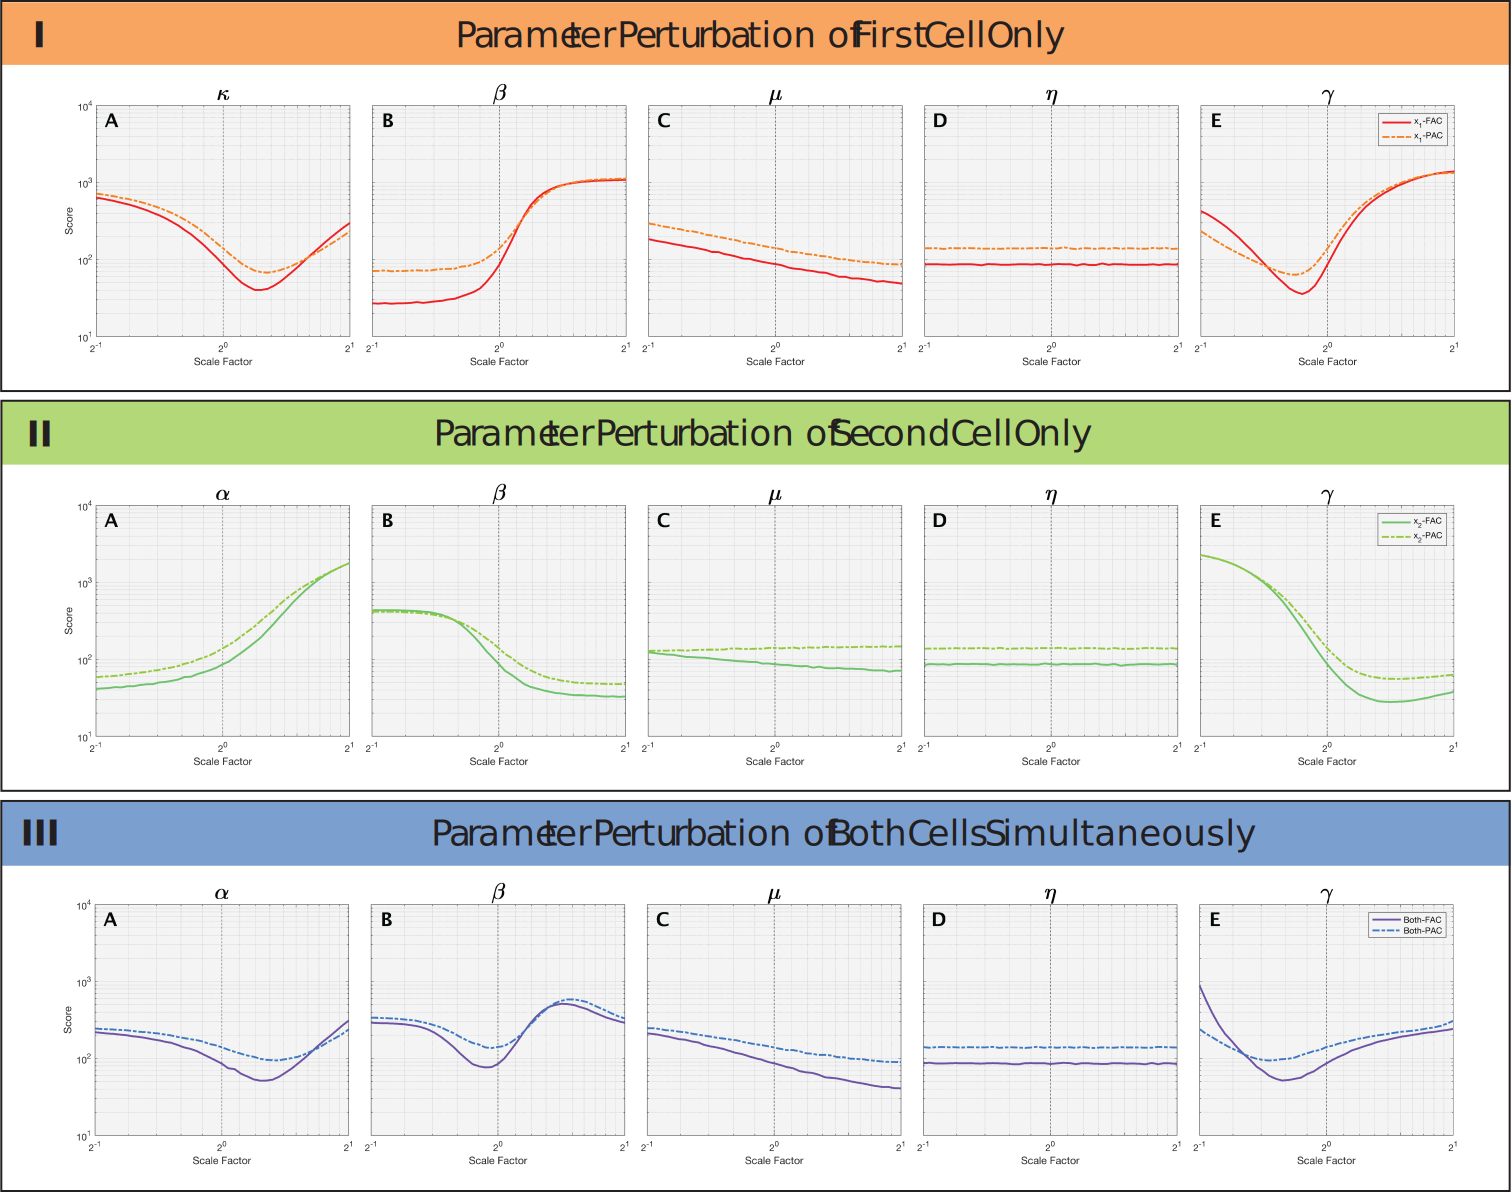
\includegraphics[width=1\textwidth]{ParameterPerturbation.pdf}
\caption{Parameter sweeps using the FAC and PAC show a broad range of control performance in cell 1 ({\bf A}),  in cell 2 ({\bf B}), and in both cells ({\bf C}). Columns show each parameter in the model, rows show the cell which has its parameter perturbed. }
\label{Parameter}
\end{center}
\end{figure*}

Real stochastic processes always have unknown or uncertain mechanisms and parameter values, and although model structures and parameter estimates can often be obtained through fitting to training data, these estimates will never be perfect due to unavoidable measurement errors or limited data sets. 
Furthermore, even with plentiful and precise training data, model and parameter uncertainties are inevitable due to the fact that even genetically identical single-cells exhibit heterogeneity in parameters due to extrinsic variations.
To asses the control performance under such parameter errors, we performed sensitivity analysis on each model parameter for each cell, then on both cells simultaneously. 
For each parameter, both the $\mathbf{u}^{\rm FAC}$ and $\mathbf{u}^{\rm PAC}$ controllers were examined across a parameter perturbation range from one-tenth to ten-fold of the original values.
Figure \ref{Parameter}A shows the results for these parameter sweeps when a single parameter in Cell 1 is varied (all other parameters are fixed), and Fig.\ \ref{Parameter}B shows the control performance as single parameters in Cell 2 is varied. 
Finally, \ref{Parameter}B shows the performance change when a single parameter is changed simultaneously in both Cell 1 and Cell 2 at the same time while keeping other parameters fixed.
In each case the baseline parameters is denoted as a vertical dashed line, and lower values of J (Eq. \ref{XXX}) denote improved performance. 
Solid lines are used to show the performance using the fully aware controller (FAC) that has access to both cells, and the dashed lines show the performance for the partially aware controller (PAC) that only has access to Cell 1.

Modification of parameters was found to produce a broad range of effects. 
For example, increasing $\beta$ in Cell 1 quickly worsens performance while increasing $\beta$ in Cell 2 improves performance (compare second column in Fig.\ \ref{Parameter}A and \ref{Parameter}B). 
In some cases, the effects on performance are not monotonic; for example, increasing $\kappa$ in Cell 1 (Fig.\ \ref{Parameter}A, leftmost column) would be highly advantageous up to a limit after which the control performance degrades rapidly. 
In other cases (such as for the promoter leakage rate, $k_0$), the effect of parameter perturbations on performance is insignificant even for relatively large ($s$=10) perturbations, suggesting that this parameter is not important to control performance.
Figure \ref{Parameter}C shows that even when parameters of both Cell 1 and Cell 2 are jointly changed, these changes could also improve or detract from control performance. 
In particular, the analysis shows that control performance could be improved by modifying the system design either to increase the auto-regulation promoter strength ($\kappa$) or its cooperativity ($\eta$) or to decrease the promoter binding constant ($\beta$) or the protein degradation rate ($\gamma$). 

\subsection{Controllers trained using one assumed level of granularity can remain effective at other levels of granularity.}

We next explored how the granularity of the system would affect the differential control of the process. Specifically, we define the level of granularity using the parameter $\alpha$ as described in Section \ref{sec:Scaling} and which affects the propensity functions and scoring according to equations \ref{eq:granscale}-\ref{EuclidV}. Effectively, larger $\alpha$ corresponds to systems where larger numbers of individual molecules are needed to achieve the same concentration (e.g., larger volumes), while smaller $\alpha$ corresponds to smaller population sizes (e.g., smaller volumes). We optimized the controller based on a the default assumption that $\alpha=1$, and we wished to know what would be the consequences if this same controller were to be applied to a system that has a different granularity. 

To explore this tradeoff, control performance scores for the $\mathbf{u}^{\rm FAC}$ and $\mathbf{u}^{\rm PAC}$ controllers were calculated at different levels of granularity ($\alpha$) between 0.2 and 2.0.  Figure \ref{Volume} (A - F) shows the joint probability distributions (left plots) and marginal probability distributions (right plots) of the system at a low granularity ($\alpha=0.2$), the original granularity ($\alpha=1.0$), and at an increased granularity ($\alpha=2.0$). 

As the system increases, the scale the size of the dynamics of the system becomes stretched over a larger region in state space. 
This effect can be observed in the smoothness of C with respect to A despite using the same system and the same controller. 
\brian[the previous two sentences do not make sense to me.]

The effect that granularity has on the control performance depends on two competing phenomena: First, because the controller was optimized for one granularity ($\alpha = 1$), one would expect that the controller would become worse if that granularity were in correct. However, at large granularity, we find that the opposite is true - the controller actually improves when applied to an incorrect model. The reason for this potentially surprising result, is that relative amplitude of stochastic fluctuations (i.e., the standard deviation divided by the mean) in a chemical process decrease with the inverse square root of the process scale \cite{Kampen1961}. At an extreme, as the system size increases, the dynamics converge towards a deterministic process, except for certain exceptional initial conditions lying on manifolds that separate different steady state behaviors \cite{XXX}. This creates a tradeoff in noise-induced control, where noise enables differential control but is also deleterious to maintaining desired states once they have been achieved. 

\begin{figure*}[t!]
\begin{center}
\includegraphics[width=1\textwidth]{Granularity.pdf}
\vspace{-0.1in}
\caption{Systems with increased granularity are less noisy and have better control performance. (A-C) Joint (left) and marginal (right) distributions for the FAC shows increased control performance and tighter distributions as $\alpha$ increases from 0.2 (top row) to 2.0 (bottom row) . (D-F) Joint (left) and marginal (left) distributions using the PAC controller at different levels of granularity.}
\label{Volume}
\end{center}
\vspace{-0.2in}
\end{figure*}

The noise reducing effect of granularity also improves the control performance of both controllers. Figure \ref{Volume}G shows the trend of the performance versus alpha for both the FAC (solid cyan line) and the PAC (solid magenta line) controller. This improvement in performance appears to approach a small value as the granularity goes to infinity, but since the size of the FSP increases with the square of the system size, systems much larger than $\alpha$=2 (where $\mathbf{A}_0\in \mathbb{R}^{10^4\times10^4}$) become more difficult to calculate. 
To bypass this limit in the FSP, sixteen SSA simulations were used to sample the CME of a system with a much larger volume of $\alpha$=100. Each SSA was ran for $5\times10^7$ minutes and only the last $4\times10^7$ minutes were sampled to estimate the stationary distribution and the calculate the performance score. The performance score estimates of this high granularity SSA using the FAC and PAC were 4.13 and 27.5 respectively, which are plotted as dashed lines in Fig.\ \ref{Volume}G. Although it is unclear if further performance improvements could be obtained with further increases to the system scale, for all cases considered so far, we found that both controllers monotonically improved with increased $\alpha$ and that $\mathbf{u}^{\rm FAC}$ always outperforms the $\mathbf{u}^{\rm PAC}$. 

The last property of system scale is the extended time dynamics. Fig \ref{Volume}(H) shows the time taken for control performance to reach steady state as $\alpha$ increases, we can see the control performance floor decrease due to lower intrinsic noise but the time scale taken to reach steady state increases with $\alpha$.

 % XXX - update this to explain what you see in this new figure. 

%These data suggest that increasing granularity increases steady state control performance even if the controller itself depends on noise for its implementation. Also, designing a controller to work for a system of one volume size can result in a controller that works even for another much larger volume.  This has practical significance, because it is relatively easy to search over a control law defined on a small $M\times M$ grid of states (e.g., when $M$=50 as in \cite{May2021}), but to implement the controller for a larger system which may be computationally prohibitive. This result implies that it may be possible to optimize controller using coarse-grained FSP analyses for small granularity problems and adapt these via interpolation for use with larger, more realistic systems, that exceed the computational limit of standard FSP computations.  

\subsection{Effects of Time Delays on Controller Performance}
\begin{figure*}
\begin{center}
\includegraphics[width=1\textwidth]{TimeDelay.pdf}
\vspace{-0.1in}
\caption{Stochastic simulations of the time delayed system show decreasing control performance using either the FAC or PAC. (A-C) Joint (left) and marginal distributions (right) of the at different levels of time delay for the FAC. (D-F) Joint (left) and marginal distributions(right) at three levels of time delay using the PAC.  (G) plots of RMSE control performance versus time delay for both FAC and PAC.}
\label{Time}
\end{center}
\vspace{-0.2in}
\end{figure*}
% XXX - This figure needs larger fonts for all the labels and axes. 
% MMM- Did the change
% Update panel letters as written in caption
% Add tic marks to left side of the A and C heat maps
% Fix the ref to baumschlager paper.

Feedback control can only be effective if one can quickly make measurements, compute adjustment to the control signal, and implement the needed change to the system. As the time required for any of these steps increases, control performance will be degraded, perhaps even leading to large fluctuations or instability. To explore how time delays would affect the noise-enhanced controller $\mathbf{u}^{\rm FAC}$ and $\mathbf{u}^{\rm PAC}$, we generated large sets of time-delayed stochastic simulations (see Methods) for different lengths of the time delay. Each SSA was sub-sampled for 1000 times over 10000 minutes of simulation time after a burnin period of 10000 minutes.

Figure \ref{Time} shows the joint distributions (left) and marginal distributions (right) at varying levels of time-delay, with panels A-C showing results for the FAC controller and panels D-F showing results for the PAC controller. Figure \ref{Time}G summarizes these results by plotting the score of both controllers versus the time delay. From the figures, it is clear that performance is rapidly degraded as the delay approaches and then exceeds the characteristic time scale of the process. At very small time delays (below $\tau = 0.07/\gamma = 0.0142$ min), the FAC outperforms the PAC ($J=$87 versus 146 at $\tau = 0.01/\gamma = 0.00203$ min) but at moderate time delays (above $\tau = 0.07/\gamma = 0.0142$ min) the PAC outperforms the FAC ($J=$170 versus 219 at $\tau = 0.1/\gamma = 0.0203$ min). 
% XXX - you can use the value of gamma=0.203 in Table 1 to write these in units of minutes.

This data show that time delays exceeding $0.07 / \gamma = 0.0142$ minutes is detrimental to the FAC control performance while delays beyond $0.2 / \gamma = 0.0406$ minutes are detrimental to the PAC controller. The choice of best controller depends on the level of time delay in the system. At extreme time delays, both controllers lose their asymmetry, resulting in significantly worse scores ($J = 1041$ and $931$). The control performance of a no-feedback controller was measured which required no inputs Figure\ref{Time}(G) (red line) and achieved a score of $J = 402$. These findings indicate that, for large time delays, attempting to improve control with feedback is less effective than using a no-feedback approach.

% XXX - This figure needs much larger fonts for all the labels and axes.
% MMM - Did the change
% There are errors in the parameter names.  What is 'alpha'?
% remove the A,B,C,D,E.
% replace I, II, III with A, B, C
% what is parameter $\mu$? Is that an error?  Please use $\mu$ for reaction index as in the methods section.

\begin{figure*}
\begin{center}
\includegraphics[width=1\textwidth]{DelayAndGranularity.pdf}
\vspace{-0.1in}
\caption{Stochastic simulations of the FAC driven system and PAC driven system show different failure modes at at different $(\tau,\alpha)$ pairs. (A-I)Joint probability distributions at different $[\tau,\alpha]$ pairs. $\alpha$ across columns and $\tau$ across rows. (J) Control performance measured over a domain of $(\tau,\alpha)$ pairs show good control performance when both $\alpha$ is large and $\tau$ small. (K) Trajectories where good control was expected but not observed show oscillations instead.}
\label{DG}
\end{center}
\vspace{-0.2in}
\end{figure*}

By increasing $\alpha$ we can change the characteristic of a system from being more noise-like to more deterministic-like. Similarly, increasing $\tau$ can decrease the quality of the control input. Generally, we would expect that increasing $\alpha$ would improve control performance, while increasing $\tau$ would decrease control performance. Therefore, joint changes in $\tau$ and $\alpha$ might reveal how the positive effect of system scale might be undone by the negative effect of time delay.

FAC steady state control performance was analyzed over a two dimensional domain of points $(\tau,\alpha)$ using thirty-two stochastic simulations simulated to steady state to see if the positive effect granularity could undo the effect of negative effect of time delay. Instead, noise induced oscillations were surprisingly found at certain $(\tau,\alpha)$ pairs and worse control performance was observed when system granularity increase for some $\tau$.  Joint probability distributions at certain $(\tau,\alpha)$ pairs and their control performance can be seen in Fig \ref{DG}(A-I). Control performance measured by RMSE increased as $\alpha$ increased when $\tau=100$ but not at $\tau=1$. FAC control performance Fig \ref{DG}(J) over the domain of points shows a valley region at low $\tau$, and a plateau region at large $\tau$. This suggests that increasing system scale at large time delays is not beneficial to control performance.  Trajectories at the edge of the valley Fig \ref {DG}(J)(yellow star) showed oscillatory behavior Fig \ref {DG}(K) and trajectories within the plateau show bursty behavior. 

The control performance domain Fig \ref{DG}(J) shows that low noise and high quality control inputs are both required to achieve good control. When noise is improved by increasing $\alpha$ the trajectories were observed going from very noisy to very oscillating which prevented improved control performance. Decreases in $\alpha$ should make the system respond faster and be less susceptible to time delay, but also more noisy. These competing effects in control performance can be observed in Fig \ref{DG}(J) which show that control performance is always poor at low $\alpha$.


\begin{figure*}
\begin{center}
\includegraphics[width=1\textwidth]{StaticControl.pdf}
\vspace{-0.1in}
\caption{The FAC and PAC control methods were used to optimize control inputs and probability distributions for static set points in a 2D domain.  Optimized control inputs and probability distributions were optimized using the FAC control method(A and B) or the PAC control method (C and D). (E) Domains of control performance for the FAC method over a region of static target points show regions of good control and symmetry along the dashed line. (F) Domain of control performance over a set of static control points for the PAC control method.} 
\label{CtrlP}
\end{center}
\vspace{-0.2in}
\end{figure*}

We analyzed the control performance over a domain of target points to find if some regions are easier to control than others. Stability analysis of the auto-regulated system using a moderate light input can create up to four stable points and one unstable point in the state space.  These points give rise to basins which may attract probability more easily than other points. Control performance of the stochastic system was analyzed over a domain of different set points and were optimized using more observable (FAC) or less observable (PAC) control.

Controllers were optimized over a two dimensional domain of target points $[T_1,T_2]$ between between five and forty-five using the FAC input method or the PAC input method. Figure \ref{CtrlP} (A) shows the optimized control input of the system when the target is $T=[20,25]$ after optimizing the FAC. Figure \ref{CtrlP} (B) show the steady state probability distribution of the controlled system.  Figure \ref{CtrlP} (C and D) show the optimized controller and probability distributions using the PAC method. The unstable point in the rate equation matches the unstable point near $(20,20)$ in this domain.

FAC and PAC control performance over the domain of static set points Fig\ref{CtrlP}(E) and (F) showed regions of good control in the FAC between 10 and 30 but a smaller region in the PAC. The FAC control performance was found to be symmetric along the dashed black line. The cause was found to be that symmetric pairs had control inputs which were exact transposes of each other. The unstable point of the system is known to be near [20,20] which is also a point of poor control for the FAC system with respect to local control performance. Edge regions were difficult to control, likely due to the geometry of how control inputs move the probability.

\begin{figure*}
\begin{center}
\includegraphics[width=1\textwidth]{DynamicControl.pdf}
\vspace{-0.1in}
\caption{Finite state projections of the slowly driven system demonstrate good control performance under a variety of phase and frequency scenario. (A) Schematic of the control problem shows targeting the number of protein in two cells using a dynamically changing reference point by cycling through a set of individual stable points and under synchronous, phase-lagged or frequency changes reference signal using only one control input. (B1-BN) shows the phase space of the reference time series, FSP solution, RMSE, reference phase space, and error residuals respectively for the synchronous control method. (C1-C5) Shows the same data for the phase-lagged control input. (D1-D5) Shows the same analysis for the frequency-changed control.}
\label{CR}
\end{center}
\vspace{-0.2in}
\end{figure*}

In \ref{Methods}, we developed a method to control the dynamics of a slowly changing system on a predefined path $r(x)$ by cycling through controllers at a fixed frequency. Thirty-two controllers were optimized along a pathway in order to target an in-sync reference point \ref{CR}, a phase lagged reference point \ref{CR}, or frequency separated reference point\ref{CR}(A). The synchronous signal is given by Fig \ref{CR}(B1) $r_1(x)=[20 sin(2 \pi x)+10, 20 sin(2 \pi x)+10]$, the phase lagged signal Fig \ref{CR}(C1) is given by $r_2(x)=[20 sin(2 \pi x)+10, 20 cos(2 \pi x)+10]$, and the frequency changed signal Fig \ref{CR}(D1) is given by $r_3(x)=[20 sin(2 \pi x)+10, 20 sin(6 \pi x)+10]$ using 32 steps for each controller. 

FSP simulations of cyclically driven systems were slowly driven at a frequency of $1e-4$ seconds and their medians are shown in the Fig \ref{CR}(B2, C2, and D2)(red line, blue line). The time series probability distributions of $x_1$ and $x_2$ can be seen as red clouds and blue clouds respectively. Regions with purple clouds are the exact overlap of red and blue. Error distributions of the system were taken by shifting the probability distribution from the reference point to the origin Fig \ref{CR}(B2, C2, and D2). Root mean squared error of each simulation are shown in Fig \ref{CR}(B3, C3,D3). 

Simulations show that the synchronous control performed the best with an average RSME of $6.9$ despite moving over the unstable point in the system. When the system is driven with a phase-lag the average RSME of the score increases to $8.2$ and when driven at a different frequency the average RMSE goes up to $8.6$.  
Suprisingly, the system is able to effectively control two signals to two different trajectories at different phase and frequency and using only a single control input despite the presence of noise Fig \ref{CR}(D3). Medians of the marginal distributions show good match with the desired reference signal in each control scheme Fig \ref{CR}(B4,C4, and D4), and time series trajectories of the RMSE show spikes in the control performance using any control strategy.

\begin{figure*}
\begin{center}
\includegraphics[width=1\textwidth]{Frequency.pdf}
\vspace{-0.1in}
\caption{Control performance analyzed over a domain of $f,\alpha$ pairs show worst control performance at moderate frequencies near $1e-2$ due to phase lag. Tracking reference signals when $\alpha=5$ span a range between 50 and 150 species (A). Stochastic simulations driven using a phased lagged controller at $\alpha = 5$ and low frequency show tighter control compared to $\alpha =1$ (B). Systems driven at moderate frequency show worse control performance than high frequency or low frequency (C). Control performance only of phase-lagged system only improves with increasing $\alpha$ and low $f$.}
\label{CRG}
\end{center}
\vspace{-0.2in}
\end{figure*}

Slowly responding systems driven at high frequency often exhibit poor control performance which improves as the driving frequency matches the time scale of the system.  The combination of both frequency driving and noise could be catastrophic for system control performance. Conversely, increasing granularity($\alpha$) may improve control performance but alters the system's time scale. Therefore these competing effects of system scale has not yet been analyzed.

To examine how driving frequency and system scale affects control performance, Sixty-four SSA trajectories of the phase-separated dynamic controller were simulated over a two dimensional domain of points $(\alpha,f)$ for 16 cycles after reaching steady state. For each $(\alpha,f)$ pair the average RMSE of the steady state trajectories were calculated.

Fig \ref{CRG}(A) shows the desired signal of a system when $\alpha = 4.0$, and Fig \ref{CRG}(B) shows the mean of the system response when $f=10^{-4}$. Fig \ref{CRG}(C) Shows control performance over normalized periodic time as $\alpha$ is held at $4.0$ and $f$ increases from $f=10^{-4}$ to $f=10^{-2}$ to $f=10^{-0}$ with an average RMSE of 6.2, 16.1, and 15.0 respectively. Heat maps of control performance over $(\alpha,f)$ pairs can be seen in Fig \ref{CRG} (D). RMSE control performance of 128 simulations were simulated over a range of frequency between $10^-3$ and $10^-1$ Fig \ref{CRG}(D) for 32 cycles to obtain a better measurement of the true RMSE Fig \ref{CRG}(D) at $\alpha=2.0$, $\alpha=4.0$, and $\alpha=8.0$. 

Heat maps of control performance over $(f,\alpha)$ pairs showed the worst performance at moderate $f$ near $f=10^{-2}$ and that control performance was best when both granularity was high and frequency was low. When examining poorly performing trajectories from moderate frequencies, a phase lag was observed in the system, while at very large frequencies the system did not respond at all. This phase las resulted in worse RMSE than no response at all.  Since the RMSE of the system at $\alpha=4$ is less than the RMSE of the $\alpha=1$ system, control performance improved with $\alpha$. 


\section{Conclusion}

Key results from \cite{May2021} showed that noise was a key requirement for the development of a noise-exploiting controller, and that deterministic systems could not be controlled to two different stable points if they both started at the same initial condition. As a stochastic system becomes increasingly more granular, it also becomes less noisy and more similar to its ODE solution which is known to be impossible to control to two different fates, but here, we have shown that the removal of noise through system granularity led to better control performance.  Therefore, stochastic controllers may perform work best on models which are nearly deterministic, but not quite. Unfortunately, such systems were found to take longer time to achieve steady state.

The ability to analyze the model at one system granularity apply it elsewhere might help analyze models for which the computational effort may be too large. Since the computation time of the FSP solution to the CME grows with the square of the number of states, this can cause an explosion in computational requirements for large systems. One alternative is to learn a controller at a computationally feasible number of states and apply them to large systems which cannot be solves for using the FSP. 

Parameter perturbation analysis showed that there is room to improve control performance by adjusting system parameters, and that joint optimization of the controller with the system parameters may lead to better control performance. It also shows that populations of cells where each cell might have its own parameter combination could still be reasonably controlled for small changes in parameter scale, but large changes could be detrimental.

Time delay analysis showed that increasing time delay decreased control performance. It was also found that a controller with less control information outperformed a controller with more information at higher levels of time delay. We believe this is happening because a controller with more information can afford to be more aggressive to implement its control, and time delay can cause this aggression to backfire. A controller was optimized which required no information in May et al which had a score of 402. This controller should be immune to time delay since no feedback is required for this controller. Here we saw both controllers did performed worse than 402 at very large time delay.

The control of cells to two slowly changing dynamic reference signals using a single global input by the use of a noise-exploiting controller showed good control performance for a variety of signals. These analysis could be extended to include faster frequency by numerical calculation or by alternative error-probability adjustments.


\begin{thebibliography}{10}
\providecommand{\url}[1]{#1}
\csname url@samestyle\endcsname
\providecommand{\newblock}{\relax}
\providecommand{\bibinfo}[2]{#2}
\providecommand{\BIBentrySTDinterwordspacing}{\spaceskip=0pt\relax}
\providecommand{\BIBentryALTinterwordstretchfactor}{4}
\providecommand{\BIBentryALTinterwordspacing}{\spaceskip=\fontdimen2\font plus
\BIBentryALTinterwordstretchfactor\fontdimen3\font minus
  \fontdimen4\font\relax}
\providecommand{\BIBforeignlanguage}[2]{{%
\expandafter\ifx\csname l@#1\endcsname\relax
\typeout{** WARNING: IEEEtran.bst: No hyphenation pattern has been}%
\typeout{** loaded for the language `#1'. Using the pattern for}%
\typeout{** the default language instead.}%
\else
\language=\csname l@#1\endcsname
\fi
#2}}
\providecommand{\BIBdecl}{\relax}
\BIBdecl

\bibitem{May2021}
M.~May and B.~Munsky, ``{Exploiting noise, nonlinearity, and feedback to
  differentially control multiple synthetic cells with a single optogenetic
  input},'' pp. 1--28, 2021.
eps
\bibitem{Ng2019}
A.~H. Ng, T.~H. Nguyen, M.~G{\'{o}}mez-Schiavon, G.~Dods, R.~A. Langan, S.~E.
  Boyken, J.~A. Samson, L.~M. Waldburger, J.~E. Dueber, D.~Baker, and
  H.~El-Samad, ``{Modular and tunable biological feedback control using a de
  novo protein switch},'' pp. 265--269, 2019.

\bibitem{Liu2018}
C.~C. Liu, M.~C. Jewett, J.~W. Chin, and C.~A. Voigt, ``{Toward an orthogonal
  central dogma},'' \emph{Nature Chemical Biology}, vol.~14, no.~2, pp.
  103--106, 2018.

\bibitem{Sheets2020}
M.~B. Sheets, W.~W. Wong, and M.~J. Dunlop, ``{Light-Inducible Recombinases for
  Bacterial Optogenetics},'' \emph{ACS Synthetic Biology}, vol.~9, no.~2, pp.
  227--235, 2020.

\bibitem{Groseclose2020}
\BIBentryALTinterwordspacing
T.~M. Groseclose, R.~E. Rondon, Z.~D. Herde, C.~A. Aldrete, and C.~J. Wilson,
  ``{Engineered systems of inducible anti-repressors for the next generation of
  biological programming},'' \emph{Nature Communications}, vol.~11, no.~1, pp.
  1--15, 2020. [Online]. Available:
  \url{http://dx.doi.org/10.1038/s41467-020-18302-1}
\BIBentrySTDinterwordspacing

\bibitem{Shin2020}
J.~Shin, S.~Zhang, B.~S. Der, A.~A. Nielsen, and C.~A. Voigt, ``{ Programming
  Escherichia coli to function as a digital display },'' \emph{Molecular
  Systems Biology}, vol.~16, no.~3, pp. 1--12, 2020.

\bibitem{Baumschlager2017}
A.~Baumschlager, S.~K. Aoki, and M.~Khammash, ``{Dynamic blue light-inducible
  T7 RNA polymerases (Opto-T7RNAPs) for precise spatiotemporal gene expression
  control},'' \emph{ACS synthetic biology}, vol.~6, no.~11, pp. 2157--2167,
  2017.

\bibitem{Chen2020}
\BIBentryALTinterwordspacing
S.~Y. Chen, L.~C. Osimiri, M.~Chevalier, L.~J. Bugaj, T.~H. Nguyen, R.~A.
  Greenstein, A.~H. Ng, J.~Stewart-Ornstein, L.~T. Neves, and H.~El-Samad,
  ``{Optogenetic Control Reveals Differential Promoter Interpretation of
  Transcription Factor Nuclear Translocation Dynamics},'' \emph{Cell Systems},
  vol.~11, no.~4, pp. 336----353.e24, 2020. [Online]. Available:
  \url{http://dx.doi.org/10.1016/j.cels.2020.08.009}
\BIBentrySTDinterwordspacing

\bibitem{Lillacci2018}
G.~Lillacci, Y.~Benenson, and M.~Khammash, ``{Synthetic control systems for
  high performance gene expression in mammalian cells},'' \emph{Nucleic acids
  research}, vol.~46, no.~18, pp. 9855--9863, 2018.

\bibitem{Fox2021}
\BIBentryALTinterwordspacing
Z.~R. Fox, S.~Fletcher, A.~Fraisse, C.~Aditya, and S.~Sosa, ``{MicroMator: Open
  and Flexible Software for Reactive Microscopy},'' \emph{bioRxiv}, pp. 1--9,
  2021. [Online]. Available:
  \url{http://biorxiv.org/cgi/content/short/2021.03.12.435206v1}
\BIBentrySTDinterwordspacing

\bibitem{Baumschlager2021}
\BIBentryALTinterwordspacing
A.~Baumschlager and M.~Khammash, ``{Synthetic Biological Approaches for
  Optogenetics and Tools for Transcriptional Light-Control in Bacteria},''
  \emph{Advanced Biology}, vol.~5, no.~5, p. 2000256, 2021. [Online].
  Available:
  \url{https://onlinelibrary.wiley.com/doi/abs/10.1002/adbi.202000256}
\BIBentrySTDinterwordspacing

\bibitem{Lugagne2017}
\BIBentryALTinterwordspacing
J.~B. Lugagne, S.~{Sosa Carrillo}, M.~Kirch, A.~K{\"{o}}hler, G.~Batt, and
  P.~Hersen, ``{Balancing a genetic toggle switch by real-time feedback control
  and periodic forcing},'' \emph{Nature Communications}, vol.~8, no.~1, pp.
  1--7, 2017. [Online]. Available:
  \url{http://dx.doi.org/10.1038/s41467-017-01498-0}
\BIBentrySTDinterwordspacing

\bibitem{Rullan2018}
\BIBentryALTinterwordspacing
M.~Rullan, D.~Benzinger, G.~W. Schmidt, A.~Milias-Argeitis, and M.~Khammash,
  ``{An Optogenetic Platform for Real-Time, Single-Cell Interrogation of
  Stochastic Transcriptional Regulation},'' \emph{Molecular Cell}, vol.~70,
  no.~4, pp. 745--756.e6, 2018. [Online]. Available:
  \url{https://doi.org/10.1016/j.molcel.2018.04.012}
\BIBentrySTDinterwordspacing

\bibitem{Guarino2020}
A.~Guarino, D.~Fiore, D.~Salzano, and M.~{Di Bernardo}, ``{Balancing Cell
  Populations Endowed with a Synthetic Toggle Switch via Adaptive Pulsatile
  Feedback Control},'' \emph{ACS Synthetic Biology}, vol.~9, no.~4, pp.
  793--803, 2020.

\bibitem{Munsky2012}
B.~Munsky, G.~Neuert, and A.~Van~Oudenaarden, ``{Using gene expression noise to
  understand gene regulation},'' \emph{Science}, vol. 336, no. 6078, pp.
  183--187, 2012.

\bibitem{Szymanska2015}
P.~Szyma{\'{n}}ska, N.~Gritti, J.~M. Keegstra, M.~Soltani, and B.~Munsky,
  ``{Using noise to control heterogeneity of isogenic populations in homogenous
  environments},'' \emph{Physical Biology}, vol.~12, no.~4, 2015.

\bibitem{Gillespie1992}
D.~T. Gillespie, ``{A rigorous derivation of the chemical master equation},''
  \emph{Physica A: Statistical Mechanics and its Applications}, vol. 188, no.
  1-3, pp. 404--425, 1992.

\bibitem{Gillespie1977}
D.~T. Gillespie, ``{Exact stochastic simulation of coupled chemical reactions},''
  \emph{The journal of physical chemistry}, vol.~81, no.~25, pp. 2340--2361,
  1977.

\end{thebibliography}

\end{document}

